\documentclass[runningheads]{llncs}

% --- A4 trap fix: force a true A4 MediaBox without touching the LNCS text block.
\AtBeginDocument{\pdfpagewidth=210mm \pdfpageheight=297mm}

\usepackage[T1]{fontenc}
\usepackage[utf8]{inputenc}
\usepackage{lmodern}   % scalable fonts (required for microtype expansion)
\usepackage{graphicx}
\usepackage{xcolor}
% amsmath + llncs emit one benign "Unable to redefine math accent \vec" warning
% (modern robust accents); silence just that during amsmath's load, then restore.
\makeatletter
\let\vp@oldwarn\PackageWarningNoLine
\renewcommand\PackageWarningNoLine[2]{}
\usepackage{amsmath,amssymb}
\let\PackageWarningNoLine\vp@oldwarn
\makeatother
\setlength{\emergencystretch}{1em}  % gentle: absorb tight lines in narrow columns
\usepackage{booktabs}
\usepackage{array}
\usepackage{tikz}
\usetikzlibrary{arrows.meta,positioning,fit,backgrounds}
\usepackage{microtype}
\usepackage[hidelinks,
  pdftitle={A Two-Condition Diagnostic for Decoder-Based Multi-Objective Search: When Blind Sampling Beats a Mismatched NSGA-II},
  pdfauthor={Javier Augusto Rebull-Saucedo; Yazmin Ivonne Flores-Martinez; Ra\'ul Gibran Porras-Alaniz},
  pdfsubject={MICAI 2026 Posters Track (Springer CCIS)},
  pdfkeywords={multi-objective optimization; random-key decoder; permutation encoding; Harris Hawks Optimization; constraint handling; Taguchi design of experiments; resource allocation}]{hyperref}
\usepackage{url}
\renewcommand\UrlFont{\color{black}\rmfamily}

% consistent metric/acronym capitalization
\newcommand{\HV}{\textsf{HV}}
\newcommand{\IGD}{\textsf{IGD}}

\graphicspath{{figures/}}

\newcommand{\repotag}{micai-cameraready-r1}

% indices matematicos a 7pt/6pt dentro de \scriptsize: lettering de artwork >= 6 pt
\DeclareMathSizes{7}{7}{6}{6}

\begin{document}

\title{A Two-Condition Diagnostic for Decoder-Based\texorpdfstring{\\}{ }Multi-Objective Search: When Blind Sampling\texorpdfstring{\\}{ }Beats a Mismatched NSGA-II}
\titlerunning{Two-Condition Diagnostic for Decoder-Based Search}

\author{Javier~Augusto~Rebull-Saucedo\orcidID{0009-0008-2089-5274}\thanks{Corresponding author.} \and
Yazmin~Ivonne~Flores-Martinez\orcidID{0009-0002-6848-1608} \and
Ra\'ul~Gibran~Porras-Alaniz\orcidID{0000-0002-6772-5351}}
\authorrunning{J.\,A. Rebull-Saucedo et al.}
\institute{Departamento de Ingenier\'ia El\'ectrica y Computaci\'on, Universidad Aut\'onoma de Ciudad Ju\'arez, Ciudad Ju\'arez, Chihuahua, M\'exico\\
\email{rebull@outlook.com}\\ \email{yazflores@outlook.com}, \email{raul.porras@uacj.mx}}

\maketitle

\begin{abstract}
Hard-constrained combinatorial problems are often solved by pairing a metaheuristic with a feasibility-preserving decoder, yet the true driver of performance is seldom isolated. We isolate it on a calibrated synthetic case study: allocating 140{,}000 U.S.\ employment-based visas a year under a per-country ceiling and spillover cascade---a three-objective integer programming model with five hard constraints and a first-in, first-out (FIFO) ordering convention, searched through a random-key decoder whose allocations are feasible by construction---no penalties, no repair. A controlled nine-method ladder shows why search fails. Blind random sampling beats a real-coded NSGA-II (Non-dominated Sorting Genetic Algorithm~II) and a naive multi-objective Harris Hawks optimizer, because the search they perform is \emph{degenerate}: interpolating operators barely change the decoded order, or gated acceptance freezes the population. At defaults, near-identity variation tracked below-blind performance on both budget-saturating instances; gated acceptance did so only on the visa, while its knapsack swarm won by $9.2\,\%$. We package the two measurements as a cheap a priori \emph{risk screen}, stressed with registered prospective tests: passing both screens identified promising methods, but was neither necessary nor sufficient across structures---a biased random-key genetic algorithm (BRKGA) crossover only ties blind sampling, and the mismatched genetic algorithm beats it on three of five instances. Across knapsack, traveling-salesman, flow-shop, and set-covering replications, the best ladder method passes both screens, while the mismatched algorithm's collapse below blind sampling is landscape- and configuration-specific. A Taguchi design selects the swarm's operating point; the recovered front Pareto-dominates the FIFO incumbent.

\keywords{Multi-objective optimization \and Harris Hawks Optimization \and Constraint handling \and Random-key decoder \and Permutation encoding \and Taguchi design of experiments \and Resource allocation}
\end{abstract}

%===============================================================================
\section{Introduction}
\label{sec:intro}

Each fiscal year the United States authorizes roughly 140{,}000 employment-based immigrant visas under two structural rules---a per-country ceiling and a spillover cascade across categories, both stated in Section~\ref{sec:formulation}---and processes petitions strictly first-in, first-out (FIFO) by priority date. The rules interact badly: two countries hold roughly three-quarters of demand (India $\approx 63\,\%$, China $\approx 14\,\%$) with 10--13-year waits, while the ceiling clash leaves thousands of visas unused.

This matters beyond accounting: behind every backlogged petition is a household whose relocation hinges on a priority date. The problem admits three legitimate, mutually conflicting goals: serve the longest-waiting petitions (\emph{efficiency}), reduce the disparity in mean served wait across national buckets (\emph{wait disparity}), and waste no visas (\emph{utilization}). No single allocation optimizes all three; the decision-relevant object is the set of best compromises---a Pareto front. Algorithmic assignment of people to scarce slots has been studied for refugee resettlement~\cite{bansak}; our contribution is methodological, not a new matching design.

Three things make that front hard to compute. The allocation is \emph{combinatorial} (integer visa counts for 105 country$\times$category groups under five simultaneous constraints and a FIFO ordering convention, a feasible set generalizing the NP-hard multidimensional knapsack~\cite{garey}). The objectives genuinely conflict. And the \emph{hard constraints} are unforgiving: a continuous metaheuristic naturally proposes infeasible candidates, and aggressive repair or penalties either require delicate tuning or distort the search landscape.

We address these challenges with a multi-objective adaptation of Harris Hawks Optimization (MOHHO) whose centerpiece is a \emph{feasibility-preserving decoder}. Our central contribution is methodological: a controlled, mechanistically explained account of when decoder-based search beats blind sampling, distilled into a two-condition diagnostic that a practitioner can run before committing a full experimental budget. Concretely, this paper contributes \emph{(i)}~a smallest-position-value (SPV) random-key decoder with a deterministic greedy assignment that satisfies R1--R6 \emph{by construction}; \emph{(ii)}~a calibrated synthetic case study whose recovered front dominates the FIFO incumbent; \emph{(iii)}~a Taguchi L9 selecting MOHHO's operating point, with ladder budgets matched to within $0.2\,\%$; and \emph{(iv)}~a nine-method ladder, a $2\times2$ package comparison and a direct Kendall-$\tau$ measurement through the decoder, which together yield the diagnostic below.

\paragraph{Roadmap.}
The framework is a two-part \emph{risk screen}: whether the variation operators change the \emph{decoded order}, and whether the selection avoids dominance-gated population freezing. On the visa both standard real-coded baselines fail one screen each and land below blind random sampling---the genetic algorithm because its operators barely move the decoded order, the swarm because gated acceptance freezes its population. Neither screen is necessary or sufficient across structures: an order-changing random-key crossover passes both and only ties blind sampling; the genetic algorithm fails the first and still wins on the sequencing instances; and the gated swarm fails the second yet beats blind sampling on the knapsack. Section~\ref{sec:formulation} states the problem and Section~\ref{sec:methods} the decoder, the optimizers and the protocol. Section~\ref{sec:results} builds the ladder, measures the mechanism, compares the two packages in a $2\times2$, and then tests the diagnostic on five structures in all---visa allocation, knapsack, traveling salesman, flow shop, and set covering as a registered prospective test---one representative instance each, so the claim does not rest on one domain. Sections~\ref{sec:discussion} and~\ref{sec:conclusions} give the screening protocol and delimit what it licenses.

%===============================================================================
\section{Background and Related Work}
\label{sec:related}

Harris Hawks Optimization (HHO)~\cite{heidari}, a population-based metaheuristic driven by a prey \emph{escape energy} (Section~\ref{sec:mohho}), has been extended to multiple objectives via external archives, elitist non-dominated sorting, and grid indices~\cite{choo,jangir,cerci,kusoglu}; these variants are validated mostly on continuous benchmarks, leaving their use on constrained combinatorial allocation---where feasibility, not convergence, is the binding difficulty---comparatively unexplored.

We bridge continuous search and combinatorial structure with random keys~\cite{bean}: a real vector is decoded to a feasible permutation by sorting (the SPV rule~\cite{tasgetiren}). How much an operator step changes the decoded phenotype is the classical representation-\emph{locality} question. Rothlauf~\cite{rothlauf} formalized it, and Raidl and Gottlieb~\cite{raidl} measured it for decoder-based evolutionary algorithms; our Kendall-$\tau$ measurement instantiates that lens. Their second theme, \emph{heuristic bias}, has a consequence we exploit: blind sampling through a greedy decoder is already a semi-greedy multistart in the GRASP (greedy randomized adaptive search procedure) sense~\cite{feo}, which makes it a demanding baseline rather than a trivial one. What this line of work establishes is that locality matters. What it leaves open---and what we supply---is a cheap risk screen a practitioner can run \emph{before} committing a search budget.

Biased random-key genetic algorithms (BRKGA)~\cite{goncalves,londe} rest on the same idea: their uniform crossover exists precisely because interpolating operators move keys without moving the decoded order. That acknowledges the failure mode without measuring when it bites. A general random-key optimizer pairs a decoder with any metaheuristic~\cite{chaves}; that is the paradigm we probe, varying the metaheuristic while holding the decoder fixed. Among constraint-handling families~\cite{rahimi}, penalty methods need problem-specific weights, repair can collapse diversity, and decoder approaches guarantee feasibility by construction---at the cost of searching only the decoder's image. We adopt the third and bound that cost explicitly rather than assuming it away.

NSGA-II (Non-dominated Sorting Genetic Algorithm~II)~\cite{deb} is our benchmark and the standard tool for hard allocation and scheduling~\cite{zhang}. Our finding speaks to the metaphor-centered critique of metaheuristics~\cite{aranha,sorensen}: once the operators match the representation, the choice of metaheuristic family is second-order. We tune parameters with a Taguchi orthogonal array~\cite{alrafei,montgomery} and assess fronts with the hypervolume~\cite{zitzler}, inverted generational distance and spacing~\cite{coello}, nonparametric tests~\cite{derrac}, and the $A_{12}$ effect size~\cite{vargha}.

%===============================================================================
\section{Problem Formulation}
\label{sec:formulation}

\paragraph{Data provenance.}
The instance is a \emph{calibrated synthetic} one, stated here because it bounds what every number below means. Country-level totals are anchored to published official aggregates~\cite{cato,uscis,dos}, but only India, China, the Philippines and Mexico have category-level demand in the public record; the remaining per-(country, category) split and the priority dates are a plausible synthetic disaggregation. It is realistic, not observed casework---which bounds external validity, not the internal comparison, since every method searches the same data.

\paragraph{Decision variables.}
The problem is discretized into $G = |\mathcal{C}| \times |\mathcal{J}| = 21 \times 5 = 105$ \emph{groups}, where each group $g$ pairs a country $c(g)\in\mathcal{C}$ with a category $j(g)\in\mathcal{J}$. The decision vector is
\(
\mathbf{x} = (x_1, x_2, \dots, x_G),\; x_g \in \mathbb{Z}^{+}_0,
\)
where $x_g$ is the number of visas assigned to group $g$. Each group has a demand (backlog) $n_g$ and a \emph{waiting weight} $w_g = t_{\text{now}} - d_g$, the years elapsed since its priority date $d_g$.

\paragraph{Objectives.}
We minimize three conflicting objectives:
\begin{align}
f_1(\mathbf{x}) &= \frac{\sum_{g}(n_g - x_g)\,w_g}{\sum_{g} n_g}
&&\text{unserved waiting load (efficiency),}\\
f_2(\mathbf{x}) &= \max_{c_1,c_2 \in \mathcal{C}}\bigl|\bar{W}_{c_1} - \bar{W}_{c_2}\bigr|
&&\text{max.\ disparity in mean served wait,}\\
f_3(\mathbf{x}) &= V - \textstyle\sum_{g} x_g
&&\text{wasted (unassigned) visas (utilization),}
\end{align}
where $V$ is the total visa supply and $\bar{W}_c = \big(\sum_{c(g)=c} x_g w_g\big)\big/\big(\sum_{c(g)=c} x_g\big)$ is the visa-weighted mean wait of country bucket $c$. So $f_2$ is the maximum disparity across modeled country buckets in the mean prior wait of served petitions. It measures neither service rates nor equality of opportunity. (An unserved bucket takes its worst backlog wait as $\bar{W}_c$, an anti-starvation convention. The post-hoc minimum-$f_2$ allocation serves all 21 modeled country buckets; other allocations need not do so.)

\paragraph{Constraints.}
The feasible set $\mathcal{F}$ is defined by five algebraic constraints plus the FIFO ordering convention R6:
\begin{align}
&\text{R1:}\; \textstyle\sum_{g} x_g \le V \text{ (total)}
&&\text{R2:}\; \textstyle\sum_{c(g)=c} x_g \le P_c \;\forall c \text{ (country)}\nonumber\\
&\text{R3:}\; \textstyle\sum_{j(g)=j} x_g \le K_j^{\text{eff}} \;\forall j \text{ (category)}
&&\text{R4:}\; 0 \le x_g \le n_g \;\forall g \text{ (demand)}\nonumber\\
&\text{R5:}\; x_g \in \mathbb{Z}^{+}_0 \;\forall g \text{ (integer)}
&&\text{R6:}\; \text{FIFO order within each } (c,j) \text{ queue}\nonumber
\end{align}
where $K_j^{\text{eff}}$ is the per-category cap after the spillover cascade. Concretely, the five categories are EB-1 to EB-5; the ceiling is the statutory $7\,\%$ cross-preference limit, $P_c \approx 25{,}620$ visas~\cite{uscis}, which no single country may exceed; and the cascade moves unused visas EB-4/5 $\rightarrow$ EB-1 $\rightarrow$ EB-2 $\rightarrow$ EB-3. We impose the statutory ceiling as a rigid exogenous cap in this single-year model---a modeling assumption, not a literal simulation of the statute (family-sponsored interactions are out of scope); the cascade is retained for generality but inert here, since every category is oversubscribed and $K_j^{\text{eff}}=K_j^{\text{base}}$, its pre-spillover value. The result is a three-objective integer programming model with five constraints and one ordering convention---three binding budget caps (R1--R3), with R4--R6 honored automatically by any assignment the decoder of Section~\ref{sec:decoder} constructs---whose feasible space grows combinatorially with $G$, motivating a metaheuristic. We use the standard notions of Pareto dominance, optimality, and the Pareto front~\cite{coello}; MOHHO approximates it through an external archive.

%===============================================================================
\section{Methods}
\label{sec:methods}

Figure~\ref{fig:pipeline} summarizes the experimental design: every method shares one evaluation path---proposals are decoded to feasible allocations and scored---and differs only in the search block, the isolation behind the ladder of Section~\ref{sec:nsga}.

\begin{figure}[t]
\centering
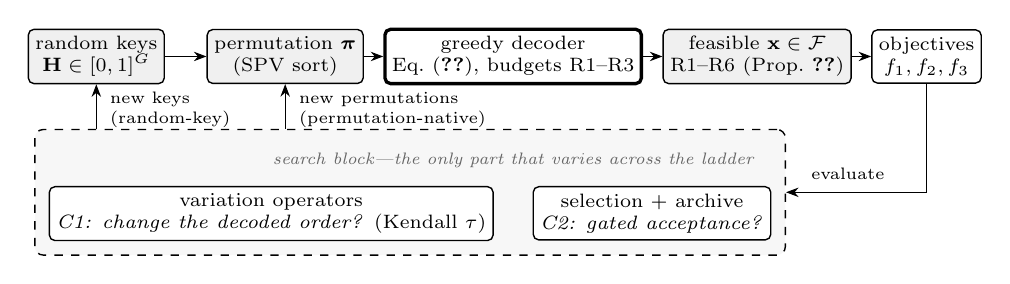
\begin{tikzpicture}[font=\scriptsize, >={Stealth[length=1.6mm]},
  box/.style={draw, rounded corners=2pt, align=center, inner sep=2.5pt,
              minimum height=15pt, line width=0.5pt},
  data/.style={box, fill=black!6},
  proc/.style={box, fill=white},
  node distance=10pt and 7pt]
% --- shared evaluation path (top row) ---
\node[data] (keys) {random keys\\$\mathbf{H}\in[0,1]^{G}$};
\node[data, right=15pt of keys] (perm) {permutation $\boldsymbol{\pi}$\\(SPV sort)};
\node[proc, very thick, right=of perm] (dec) {greedy decoder\\Eq.~(\ref{eq:greedy}), budgets R1--R3};
\node[data, right=of dec] (alloc) {feasible $\mathbf{x}\in\mathcal{F}$\\R1--R6 (Prop.~\ref{prop:feas})};
\node[proc, right=of alloc] (obj) {objectives\\$f_1,f_2,f_3$};
\draw[->] (keys) -- (perm);
\draw[->] (perm) -- (dec);
\draw[->] (dec) -- (alloc);
\draw[->] (alloc) -- (obj);
% --- search block (bottom row, swapped across the ladder) ---
\node[font=\fontsize{6.2}{7.2}\selectfont\itshape, text=black!60, below=21pt of dec.south] (blocklbl)
  {search block---the only part that varies across the ladder};
\node[proc, below=3pt of blocklbl.south, anchor=north east, xshift=-7pt] (ops)
  {variation operators\\\textit{C1: change the decoded order?} (Kendall $\tau$)};
\node[proc, below=3pt of blocklbl.south, anchor=north west, xshift=7pt] (sel)
  {selection $+$ archive\\\textit{C2: gated acceptance?}};
\begin{scope}[on background layer]
\node[draw, dashed, rounded corners=3pt, fill=black!3, inner sep=5pt,
      fit=(blocklbl)(ops)(sel), line width=0.5pt] (block) {};
\end{scope}
\draw[->] (obj.south) |- node[above=1pt, font=\fontsize{6.2}{7.2}\selectfont, pos=0.78]{evaluate} (block.east);
\draw[->] (block.north -| keys.south) -- node[right=1.5pt, pos=0.42, font=\fontsize{6.2}{7.2}\selectfont, align=left]
  {new keys\\(random-key)} (keys.south);
\draw[->] (block.north -| perm.south) -- node[right=1.5pt, pos=0.42, font=\fontsize{6.2}{7.2}\selectfont, align=left]
  {new permutations\\(permutation-native)} (perm.south);
\end{tikzpicture}
\caption{The experimental design: a shared feasibility-preserving evaluation path (top; permutation-native methods enter one step later) and the search block (bottom, shaded), the only component swapped across the method ladder. The diagnostic asks whether operators change the decoded order (C1) and whether selection avoids dominance-gated freezing (C2).}
\label{fig:pipeline}
\end{figure}

\subsection{Multi-objective Harris Hawks Optimization}
\label{sec:mohho}

Each hawk is a position $\mathbf{H}\in\mathbb{R}^{G}$ in the box $[0,1]^{G}$ (here $G=105$). At iteration $t$ the escape energy is
\begin{equation}
E = 2E_0\!\left(1 - \tfrac{t}{T}\right), \qquad E_0 \sim U(-1,1),
\label{eq:energy}
\end{equation}
which drives the choice among six movement operators, selected by $|E|$ and two uniform draws: two exploration moves ($|E|\ge1$; relative to a random hawk or to the population centroid), a soft and a hard besiege toward the prey ($0.5\le|E|<1$ and $|E|<0.5$), and a L\'evy-dive variant of each besiege. The multi-objective adaptation draws the \emph{leader} (the ``rabbit'' of the HHO metaphor) from an external archive of non-dominated solutions with probability proportional to crowding distance, prunes the most crowded solution on overflow, and updates the archive after every move; archive size is tuned in Section~\ref{sec:taguchi}. A hawk moves solely when its trial dominates its current position (single-objective HHO's greedy replacement lifted to dominance; the published variants~\cite{jangir,cerci,kusoglu} do not specify this acceptance, so the naive configuration's failures characterize this choice). For evaluation fairness, the L\'evy operators accept a single trial point per hawk per iteration (canonical HHO evaluates two), so MOHHO, like every method, consumes $N\times T$ offspring evaluations.

\paragraph{Why this optimizer.}
We do not present HHO as a state-of-the-art multi-objective method, and no step of the argument needs it to be one; it enters as a \emph{representative swarm baseline}. Its published multi-objective variants leave the acceptance rule unspecified, and the natural lift of single-objective HHO's greedy replacement---move only on domination---is exactly the gated acceptance our second condition is about. That makes it the cheapest instance of a search whose population freezes while its operators keep proposing. The dominance, decomposition and strength-Pareto methods a reader would expect---NSGA-II, MOEA/D and SPEA2---are all in the ladder. We make no claim that the swarm is best; it enters as a control on the acceptance rule, not as a contender.

\subsection{A feasibility-preserving decoder}
\label{sec:decoder}

The HHO operators act in the continuous space $\mathbb{R}^{G}$, but the problem is combinatorial with five hard constraints and a FIFO ordering convention. We bridge the two with the SPV rule~\cite{bean,tasgetiren}---which turns a hawk $\mathbf{H}$ into a permutation $\boldsymbol{\pi}$ by sorting the group indices in ascending order of their key $h_g$ (component $g$ of $\mathbf{H}$)---followed by a deterministic greedy assignment (Figure~\ref{fig:pipeline}) that walks the groups in SPV order and fixes the model's decision variable
\begin{equation}
x_g = \min\!\bigl(n_g,\; V^{\text{rem}},\; P^{\text{rem}}_{c(g)},\; K^{\text{rem}}_{j(g)}\bigr),
\label{eq:greedy}
\end{equation}
decrementing the residual budgets of R1--R3 (initialized to $V$, $P_c$, and $K_j^{\text{eff}}$) after each step. No penalties, no repair: the hawks search directly on a feasible landscape. The greedy fill is budget-saturating (each visited group gets its maximal feasible amount), so the decoder's image is the saturating subset of $\mathcal{F}$ and all dominance claims are relative to it; an exact bi-objective $(f_1,f_3)$ mixed-integer linear program (MILP), reported with the robustness checks below, tests whether that subset loses anything relevant.

\begin{proposition}[Feasibility by construction]
\label{prop:feas}
For any hawk $\mathbf{H}\in\mathbb{R}^{G}$, the allocation $\mathbf{x}$ returned by the SPV${}+{}$greedy decoder satisfies R1--R6.
\end{proposition}

\begin{proof}
Each step caps $x_g$ by every remaining budget and by $n_g$, so by induction every residual stays $\ge 0$ (R1--R3), while $0\le x_g\le n_g$ gives R4 and integrality gives R5; serving each group's $x_g$ most-senior petitions honors R6. \qed
\end{proof}

\subsection{Benchmarks and a representation-matched optimizer}
\label{sec:nsga}

The \emph{ladder} shares the greedy decoder, the objectives, the hypervolume reference point and an approximately $25{,}000$-evaluation budget, matched to within $0.2\,\%$ rather than exactly: blind random restart draws $25{,}000$ candidates, the population-based methods spend $25{,}050$ including the initial population, and permutation-MOEA/D spends $25{,}020$ over its $45$ weight vectors. All nine run for 30 seeds (1--30); external archives, where applicable, hold 100 solutions.

Three methods act on the continuous SPV random keys in $\mathbb{R}^{G}$: \emph{(a)}~the MOHHO of Section~\ref{sec:mohho}; \emph{(b)}~NSGA-II~\cite{deb} with simulated binary crossover (SBX, $\eta_c=20$, $p_c=0.9$), polynomial mutation ($\eta_m=20$, $p_m=1/d$ for search-space dimension $d$), binary tournament selection and elitist $(\mu+\lambda)$ replacement; and \emph{(c)}~random restart, drawing every candidate uniformly at random (the decoder alone).

Four act directly on permutations of the 105 groups, decoded by the same greedy procedure, and span four paradigms: \emph{(d)}~permutation-NSGA-II (dominance) with order crossover (OX) and swap mutation; \emph{(e)}~permutation-MOEA/D (decomposition~\cite{zhangli}; Tchebycheff over 45 weight vectors, neighborhood 10, same OX${}+{}$swap); \emph{(f)}~permutation-SPEA2~\cite{spea2} (strength-Pareto, density-based truncation) under the same operators; and \emph{(g)}~Discrete-MOHHO, which keeps HHO's escape energy of Eq.~(\ref{eq:energy}) and its crowding-pruned archive but expresses every move on permutations (OX with a random hawk or the leader, $|E|$-scaled swaps, occasional segment reversals). Discrete HHO variants exist for single-objective settings~\cite{gezici}.

Two further random-key methods vary one mechanism each. \emph{(h)}~rk-NSGA-II (biased uniform)~\cite{goncalves} is the skeleton of method~(b) with SBX and polynomial mutation replaced by BRKGA-style parameterized uniform crossover (elite-parent gene with probability $\rho_e=0.7$) and per-gene random-reset mutation. \emph{(i)}~NDS-selected MO-HHO---we write MOHHO for the dominance-gated swarm of \emph{(a)} and MO-HHO for this variant---keeps HHO movement but replaces dominance-gated acceptance by elitist non-dominated sorting (NDS) with crowding, adds an SBX step toward the leader ($p_c=0.9$, $\eta_c=15$) and polynomial mutation ($p_m=0.15$, $\eta_m=20$), and prunes its archive at 100.

\subsection{Evaluation protocol, indicators, and tuning}
\label{sec:protocol}

We assess each front with four indicators. The \emph{hypervolume} (\HV; larger is better) uses a fixed \emph{historical empirical reference point} $(10;\,16;\,20{,}000)$, shared by every method and not a certified bound: it dominates $15{,}270$ of the $15{,}273$ points in the $9\times30$ per-run fronts, the three exceptions being MOHHO solutions with $f_3\ge 20{,}000$ (largest $20{,}200$), which the indicator discards. The \emph{inverted generational distance} is $\IGD(F)=|Z|^{-1}\sum_{z\in Z}\min_{a\in F}\lVert a-z\rVert$ (smaller is better) against a reference front $Z$; its dominance-compliant variant \IGD$^{+}$ replaces $\lVert a-z\rVert$ by $\lVert\max(a-z,0)\rVert$. \emph{Spacing} is the standard deviation of nearest-neighbor distances within a front and \emph{cardinality} its size; objectives are min--max normalized before all three. Three reference fronts are kept apart: $Z_2$ ($126$ points, MOHHO${}\cup{}$NSGA-II) for that pairwise comparison; $Z_9$ ($185$), the non-dominated union of the current $9\times30$ per-run fronts, which also supply the reference-point coverage count above; and $Z_{9,\text{hist}}$ ($187$), its earlier counterpart, for the historical \IGD$^{+}$/$\epsilon$ re-scoring of Section~\ref{sec:ablation}. Sensitivity to that choice---a one-directional sweep over looser $f_3^{\text{ref}}$, whose first fully dominating value is $20{,}201$ and which runs to $25{,}000$, together with a three-coordinate sweep that also tightens it---yields the five reference points whose effect on the tier ordering Section~\ref{sec:ablation} reports.

Each algorithm runs for 30 independent seeds; a \emph{combined front} is the non-dominated union of its 30 per-run fronts. A shared seed label does not couple two methods---different representations consume the stream differently, and a common instance, decoder and budget are constants, not a source of covariance---so we treat runs as independent replicates and reserve paired tests for the two designs where blocking is real. For algorithm-versus-algorithm contrasts the unpaired Mann--Whitney $U$~\cite{derrac} is primary and the seed-label Wilcoxon is the sensitivity, two-sided unless noted; the order reverses where blocking is real---the $2\times2$, whose cells share an initial population, and the preregistered mo-SCP test. For the ladder as a whole the primary omnibus is Kruskal--Wallis, with a seed-label Friedman and a Nemenyi post-hoc~\cite{demsar} as descriptive sensitivity. Holm corrects across an enumerated family of twelve headline claims (Section~\ref{sec:ablation}), computed once with the unpaired tests and once with the seed-label and blocked ones; all twelve survive under both. Effect size is the Vargha--Delaney $A_{12}$~\cite{vargha}, reported per method in Table~\ref{tab:ladder}. The deterministic FIFO baseline decodes groups in ascending priority-date order: $f_1=8.7891$, $f_2=13.0$ years, $f_3=1{,}940$ wasted visas.

%===============================================================================
\paragraph{Parameter tuning.}
\phantomsection\label{sec:taguchi}%
We replace empirical parameter choices by a Taguchi L9$(3^4)$ orthogonal-array design~\cite{alrafei,montgomery} over four factors at three levels: population $N\in\{30,50,70\}$, iteration budget $T\in\{100,300,500\}$, archive size $\in\{50,100,150\}$, and L\'evy exponent $\beta\in\{1.3,1.5,1.7\}$. The response is the larger-the-better signal-to-noise (S/N) ratio of the hypervolume, with each of the nine configurations replicated over 12 seeds disjoint from the evaluation seeds.

Averaging S/N per factor level gives an unambiguous ranking: population ($\Delta=0.318$~dB) and iteration budget ($\Delta=0.155$~dB) dominate, while $\beta$ ($0.108$~dB) and archive size ($0.046$~dB) lie within run-to-run noise. The additive model predicts the optimum $N{=}70$, $T{=}500$ at S/N $\approx109.77$~dB; a confirmation run gives $109.66$~dB ($\HV=304{,}391$), validating the model. The 30-run study adopts a conservative, compute-economical operating point: $N{=}50$, $T{=}500$, archive $100$, $\beta{=}1.5$. Its confirmation gives S/N $109.56$~dB---within $1.2\,\%$ in hypervolume of the L9 optimum, which differs only in $N{=}50$ vs.\ $70$.

Two choices deserve stating. The L9 selects MOHHO's operating point over population, budget, archive size and $\beta$; the ladder then matches budgets to within $0.2\,\%$ rather than sharing a tuned configuration. The permutation-native methods inherit that point with no tuning study of their own, which is conservative rather than favorable to our reading. Where per-method tuning could plausibly overturn a result we ran it anyway---NSGA-II's own L9, on the visa and the knapsack---and report both outcomes in Section~\ref{sec:ablation}.

%===============================================================================
\section{Results}
\label{sec:results}

\subsection{Combined Pareto front and domination of FIFO}
\label{sec:front}

Combining and re-filtering the 30 runs yields a front of 104 non-dominated solutions (Figure~\ref{fig:pareto2d}); the FIFO baseline is Pareto-dominated. The extreme solutions expose the trade-offs: minimum wait disparity (minimum-$f_2$: $f_1=8.9994$, $f_2=2.0$~yr, $f_3=0$), full utilization (minimum-$f_3$: $8.996$, $2.46$, $0$), and the minimum-$f_1$ solution that dominates FIFO---strictly better on waste ($f_3$ from 1{,}940 to 680 visas), tied on the maximal disparity ($f_2=13.0$), and negligibly better on the near-degenerate $f_1$ (8.7891 to 8.7884). The substantive case against FIFO is thus about waste and wait disparity: 94 of the 104 front solutions reach $f_3=0$ (zero waste, which FIFO never attains), with disparities spanning from 13.0 years down to 2.0. (The MOHHO, Discrete-MOHHO, and permutation-NSGA-II combined fronts agree within $0.3\,\%$ in hypervolume.) Convergence is fast: mean hypervolume reaches 99\,\% of its final value by iteration~135, and over the 30 runs the \HV\ distribution is narrow (mean $302{,}756$, coefficient of variation [CV] $2.36\,\%$).

\begin{figure}[t]
\centering

\includegraphics[width=0.50\textwidth]{pareto_f1f2.pdf}
\caption{The $f_1$--$f_2$ projection of the 104-solution combined Pareto front, colored by the third objective $f_3$ (wasted visas). The FIFO baseline (star) is Pareto-dominated; its own $f_3=1{,}940$ lies beyond the color scale.}
\label{fig:pareto2d}
\end{figure}

\subsection{Decoder, representation, and search: a controlled ladder}
\label{sec:ablation}

The ladder results (Table~\ref{tab:ladder}, Figure~\ref{fig:ladder}) attribute performance to its true source; the permutation-native methods run under approximately the same budget with no method-specific tuning. Under this budget MOHHO beats the real-coded NSGA-II by $3.2\,\%$ in mean hypervolume (Mann--Whitney $p=3.6\times10^{-6}$; seed-label Wilcoxon $p=4.4\times10^{-6}$; $A_{12}=0.85$) and its combined front is more evenly spread (spacing $0.011$ vs.\ $0.046$), while NSGA-II edges it on \IGD\ against $Z_2$ ($0.007$ vs.\ $0.021$)---the two indicators the ladder does not rely on, reported here because both fronts are scored under one protocol.

\paragraph{Blind sampling beats near-identity search---but not an NDS-selected swarm.}
\emph{Random restart}---blind sampling with no search---lands $5.7\,\%$ above the real-coded NSGA-II and $2.5\,\%$ above the classic real-coded MOHHO (Table~\ref{tab:ladder}) (the naive swarm has higher \HV\ in only $10/30$ seed-label comparisons). Giving NSGA-II MOHHO's archive barely helps ($293{,}666$ vs.\ $293{,}367$).

Nor is blind sampling's strength order-level greediness: a GRASP-style semi-greedy control~\cite{feo} ($\alpha\sim U(0,1)$, same budget) lands $3.8\,\%$ below uniform constructions ($298{,}531$, Mann--Whitney $p=6.1\times10^{-11}$)---the decoder's heuristic bias~\cite{raidl} helps every construction. Nor is it tuning: NSGA-II's own L9 (best confirmed on the 30-seed block: $\eta_c{=}2$, $p_m{=}5/d$) climbs to $308{,}082$, a statistical tie with blind sampling (Mann--Whitney $p=0.15$), still $3.2\,\%$ below the permutation tier; a Pareto local search (single swaps are near-identity, so the first screen flags it) lands $2.0\,\%$ below blind sampling (Mann--Whitney $p=1.9\times10^{-4}$). Five controls---archive, semi-greedy construction, tuning, local search and the registered sweep---tell one story: nothing we tested short of order renewal beats blind sampling here.

Method~\emph{(i)}, the NDS-selected MO-HHO, shows that what fails is degenerate search rather than real-coded search as such. An implementation correction applied after the preregistered outcome brought its archive capacity from 200 to the common 100; it moved its mean hypervolume by less than $0.001\,\%$ and altered no inference, and both artifacts are retained. It recovers at least $0.99$ of the true-front hypervolume on the bi-objective ZDT1/ZDT2 benchmarks, where the naive swarm collapses to $0.20$ on ZDT2, but only $0.885$ on the tri-objective DTLZ2---consistent with stronger archive truncation. We therefore use it as a selection-mechanism control, not as a universally validated optimizer. On the visa it beats random restart ($316{,}345$ vs.\ $310{,}214$, $+2.0\,\%$, one-sided Mann--Whitney $p=5.9\times10^{-5}$; seed-label Wilcoxon $p=5.7\times10^{-4}$; 30 seeds).

\paragraph{Why near-identity operators fail.}
We measured why real-coded NSGA-II falls below blind sampling. On the SPV random keys, SBX and polynomial mutation are near-identity on the decoded permutation: over $3{,}000$ trials the Kendall rank correlation between a parent's SPV order and its child's is $\tau=0.99$ (and stays in $[0.987,0.992]$ along the search trajectory). Sweeping the crossover distribution index $\eta_c\in\{2,5,10,20,50,100\}$ confirms this is no tuning artifact: even the most disruptive setting ($\eta_c{=}2$, $\tau{=}0.92$) leaves the GA's mean \HV\ at $305{,}293$, below blind random restart---the GA perturbs the keys so little that the induced permutation barely changes, leaving it almost frozen in combinatorial space. HHO's position updates, by contrast, propose large permutation jumps ($\tau\approx0$) that the dominance-gated acceptance rarely admits (only ${\sim}0.6\,\%$ of hawks move per iteration), but the archive keeps the rejected proposals---hence MOHHO $>$ NSGA-II within the random-key tier. The real-coded MOHHO is thus a deliberately standard, weak baseline (its ZDT2 collapse persists under every acceptance rule and repair we tried): the thesis rests on degenerate search losing even to blind sampling, not on swarm strength.

\paragraph{Matching the operators to the representation.}
The clean fix is to act directly on permutations, lifting four distinct paradigms above blind sampling---permutation-NSGA-II (dominance/GA), permutation-SPEA2 (strength-Pareto), Discrete-MOHHO (swarm), and permutation-MOEA/D (decomposition)---and the NDS-selected random-key swarm joins them (Table~\ref{tab:ladder}), so the encoding is not the divider. The four cluster within about $1\,\%$ of one another (permutation-SPEA2 vs.\ permutation-NSGA-II: Mann--Whitney $p=0.47$, seed-label Wilcoxon sensitivity $p=0.24$---a statistical tie either way), yet all sit $1.5$--$2.6\,\%$ above blind random restart. Discrete-MOHHO improves on classic MOHHO by $+4.6\,\%$ (one-sided Mann--Whitney $p=1.4\times10^{-10}$; seed-label Wilcoxon $p=9.3\times10^{-10}$; better on all $30/30$ seeds); the most stable methods are matched ones (permutation-NSGA-II CV $0.58\,\%$, Discrete-MOHHO $0.71\,\%$, vs.\ classic MOHHO $2.36\,\%$), permutation-NSGA-II leading Discrete-MOHHO by $+0.43\,\%$ in mean \HV. Made representation-matched, the swarm reaches the top tier with low variance---a mechanism check rather than a champion claim (replacing its energy schedule by run-average constants shifts \HV\ by $+0.01\,\%$, $p=0.87$: the metaphor's scheduling is not a measurable driver here~\cite{aranha,sorensen}).

\paragraph{The two screens, graded by a prospective test.}
The ladder suggests a two-part screening pattern for this landscape: whether the operator changes the decoded order ($\tau$ far from $1$), and whether the selection avoids dominance-gated acceptance (non-dominated sorting, strength-Pareto, decomposition or a crowded archive are architectures intended to keep the population from freezing; we measure the freezing, not the diversity). NSGA-II fails the first; the naive MOHHO fails the second; the NDS-selected MO-HHO and all four permutation-native methods pass both and beat random restart here. We tested the rule on a method not used to formulate it: the rk-NSGA-II (biased uniform) of Section~\ref{sec:nsga}, whose BRKGA-style crossover changes the decoded order ($\tau=0.63\pm0.07$) under unchanged selection. Read as a binary conjunction the screen would flag it as promising; it is not. The method's mean \HV\ of $309{,}970$ is a statistical tie with random restart ($310{,}214$; Mann--Whitney $p=0.74$, $A_{12}=0.47$); a canonical BRKGA ($20\,\%$ elites, $15\,\%$ mutants, same crossover) lands at the same level ($309{,}928$). So passing both screens is not sufficient. Within the random-key GA family, holding selection fixed and varying the variation package gives an ordered three-point sequence in the measured order-preservation---$\tau{=}0.99\!\to\!293{,}367$; $\tau{=}0.92\!\to\!305{,}293$; $\tau{=}0.63\!\to\!309{,}970$---and the HHO-move package of Section~\ref{sec:twoconditions} reaches $315{,}730$ under the same selection, although its own $\tau$ was not measured. A registered sweep (predictions committed before running: $\rho_e$ at eleven levels spanning $\tau\in[0.42,1.0]$, fixed selection, all five structures, 30 seeds per level) shows a family contrast, not a dose--response: hypervolume is nearly flat in $\tau$ on every structure (Spearman $\rho$ from $-0.07$ to $0.48$, n.s.), while \IGD$^{+}$ (the dominance-compliant variant), against the pooled sweep front, degrades as $\tau\to1$ on three of the five ($\rho\ge0.80$). So $\tau$ is a flag, not a dial; only a coverage metric sees the residual dose effect.

\paragraph{An empirical regularity.}
That encoding--operator mismatch can hurt search has been known since random keys were introduced~\cite{bean}, with the locality of decoder-based encodings formalized by Rothlauf~\cite{rothlauf} and measured by Raidl and Gottlieb~\cite{raidl}; our contribution is the controlled, multi-method, graded demonstration on a realistic constrained problem---including that both default real-coded baselines fall below blind sampling. Within a matched representation operator set and selection architecture are second-order (a $3\times3$ factorial attributes them only $5.5\,\%$ and $13.4\,\%$ of the hypervolume variance, against $78\,\%$ seed noise). A Kruskal--Wallis omnibus across all nine ladder methods rejects equal performance decisively ($H=149.8$, $p\approx2.1\times10^{-28}$); the seed-label Friedman with a Nemenyi post-hoc~\cite{demsar} agrees as descriptive sensitivity ($\chi^2=133.8$, $p\approx4.6\times10^{-25}$, critical difference $2.19$) and gives the following descriptive seed-label ranks (permutation-NSGA-II $2.97$ best, real-coded NSGA-II $8.77$ worst; rk-NSGA-II $4.57$, within the critical difference of random restart $6.47$); all twelve headline claims survive Holm (six ladder contrasts against blind random restart; MOHHO vs.\ NSGA-II; Discrete-MOHHO vs.\ MOHHO; the winning $2\times2$ cell; the $2\times2$ interaction; and the two prospective mo-SCP contrasts), and an independent re-scoring of a stored archive of per-run fronts against $Z_{9,\text{hist}}$, under \IGD$^{+}$ and additive $\epsilon$, keeps four of the five top-tier methods in the top four ranks (permutation-MOEA/D is the one displacement; rank correlations $0.82$/$0.85$ with \HV). That archive reproduces the Table~\ref{tab:ladder} runs exactly for six of the nine methods; for the other three it comes from a separate execution differing by at most $0.13\,\%$ in mean \HV, so we read it as a robustness check on the indicator, not a re-scoring of the same runs. What the ladder establishes is an empirical regularity for this problem, not a general law.

\begin{table}[t]
\centering
\caption{The method ladder: 30 runs each, identical greedy decoder and a matched ${\approx}25{,}000$-evaluation budget. Top block: random-key encoding; bottom block: permutation-native. $\sigma$ denotes the population standard deviation over 30 runs. $A_{12}$ is the Vargha--Delaney effect size against blind random restart ($0.5$: no difference). Best per column in bold; rk-NSGA-II's best combined \HV\ reflects between-run dispersion, not per-run strength. $|F|$: solutions in the combined front; ``perm-'' abbreviates ``permutation-'', ``NDS-sel.'' the NDS-selected real-coded MO-HHO.}
\label{tab:ladder}
\footnotesize
\begin{tabular}{llccrrc}
\toprule
\textbf{Method} & \textbf{Paradigm} & \textbf{Mean \HV\ $\pm\,\sigma$} & \textbf{CV} & \textbf{Comb.\ \HV} & \textbf{$|F|$} & \textbf{$A_{12}$}\\
\midrule
NSGA-II            & GA       & $293{,}367 \pm 6{,}996$ & 2.38\,\% & 316{,}060 & 92 & 0.027\\
MOHHO              & swarm    & $302{,}756 \pm 7{,}138$ & 2.36\,\% & 320{,}984 & 104 & 0.254\\
rk-NSGA-II (biased)  & GA & $309{,}970 \pm 9{,}790$ & 3.16\,\% & \textbf{325{,}465} & 157 & 0.474\\
Random restart     & ---      & $310{,}214 \pm 2{,}735$ & 0.88\,\% & 317{,}673 & 65 & ---\\
NDS-sel.\ MO-HHO   & swarm    & $316{,}345 \pm 6{,}682$ & 2.11\,\% & 321{,}799 & \textbf{204} & 0.790\\
\midrule
perm-MOEA/D                 & decomp.\ & $314{,}846 \pm 5{,}384$  & 1.71\,\% & 320{,}969 & 90 & 0.860\\
Discrete-MOHHO              & swarm    & $316{,}792 \pm 2{,}258$  & 0.71\,\% & 321{,}408 & 137 & 0.972\\
perm-SPEA2                  & str.-Pareto & $317{,}135 \pm 3{,}814$ & 1.20\,\% & 322{,}037 & 179 & 0.961\\
perm-NSGA-II                & GA       & $\mathbf{318{,}151 \pm 1{,}855}$ & \textbf{0.58\,\%} & 321{,}935 & 148 & \textbf{0.999}\\
\bottomrule
\end{tabular}
\end{table}

\begin{figure}[t]
\centering

\includegraphics[width=0.71\textwidth]{ladder.pdf}
\caption{The nine-method ladder: per-run hypervolume (30 runs each, identical decoder and budget). The divider is non-degenerate search, not the encoding: the BRKGA-style rk-NSGA-II only ties blind random restart; the NDS-selected MO-HHO joins the top tier.}
\label{fig:ladder}
\end{figure}

\paragraph{Robustness to a search-space-collapse confound.}
Three checks bound budget saturation as a confound. \emph{Structure}: $50{,}000$ random permutations yield $39{,}401$ distinct objective points (degeneration ratio $1.27$); a principal-component analysis puts about $99\,\%$ of the front variance in two components and $0.81$--$0.91$ in the first, exposing one wide $f_2$ axis. \emph{Decoder}: with two non-saturating feasibility-preserving decoders, the permutation tier remains above the random-key tier (one-sided Mann--Whitney $p<10^{-4}$; one-sided seed-label Wilcoxon $p<10^{-3}$), while the margin shrinks from $6.9\,\%$ under greedy to $4.3\,\%$ under stochastic-skip and $1.4\,\%$ under fractional-intensity. An exact $(f_1,f_3)$ MILP projection finds no practically meaningful non-saturating solution missed by greedy; $f_2$ is evaluated a posteriori because it is outside that MILP form. \emph{Metric}: the per-run tier ordering survives four of five reference points, although combined-front tiers soften under reference-free metrics. Thus saturation amplifies rather than creates the modest visa-instance effect; generalization is examined below.

\subsection{Comparing the two packages: a controlled $2\times2$}
\label{sec:twoconditions}
The ladder establishes the two screens by observation; we compare four complete packages on a single real-coded random-key skeleton---same greedy decoder, instance, $25{,}050$-evaluation budget and 30 seeds. The first factor is the \emph{variation package}: HHO moves with polynomial mutation ($p_m=0.15$) against SBX ($\eta_c=20$) with polynomial mutation ($p_m=1/105$). The second is the \emph{selection rule}: elitist non-dominated sorting (NDS) with crowding against dominance-gated acceptance. Of the four packages (Figure~\ref{fig:mech2x2}), only HHO${}+{}$polynomial mutation under NDS beats blind random restart ($315{,}730$ vs.\ $310{,}214$~\HV, $+1.78\,\%$, $A_{12}=0.79$); the other three fall below it, losing by $1.4$--$2.0\,\%$. The four cells share their initial population by construction, so blocking is genuine and the paired test is primary (one-sided Wilcoxon $p=1.4\times10^{-3}$). Gated acceptance freezes the population: only $0.87\,\%$ and $1.75\,\%$ of offspring dominate and replace their parent per iteration in the two gated cells. A blocked difference-in-differences contrast finds a package${}\times{}$selection interaction (Wilcoxon on the within-seed contrast, $p=7.979\times10^{-4}$; a within-block sign-flip permutation agrees, $p=6.0\times10^{-4}$): the two factors do not simply add.

\begin{figure}[t]
\centering

\includegraphics[width=0.70\textwidth]{mechanism_2x2_annot.pdf}
\caption{The controlled $2\times2$, both factors categorical: the variation package (C1) against the selection rule (C2). Each cell carries mean hypervolume, gap to blind random restart (\HV\ $310{,}214$), and the Vargha--Delaney effect size, printed \texttt{A12} inside the panel. Only HHO${}+{}$polynomial mutation under NDS (circle) beats blind sampling. The replacement fraction is the proportion of offspring that dominate and replace their corresponding parents; under non-dominated sorting the next population is selected from the parent--offspring union, for which that parentwise statistic is not defined, so it is shown only for the gated cells.}
\label{fig:mech2x2}
\end{figure}

\subsection{Generalization}
\label{sec:secondproblem}

\paragraph{Perturbed-demand instances.}
Across five $\pm20\,\%$ demand perturbations (10 fixed seeds each; caps recomputed), FIFO remains dominated, MOHHO exceeds NSGA-II in all five (two individually significant, one-sided Mann--Whitney), and random restart reaches $101$--$103\,\%$ of MOHHO. These checks are descriptive, not confirmatory.

\paragraph{Structurally distinct problems.}
We replicate the six-method core of the ladder on three classic structures sharing only the SPV${}+{}$greedy/permutation methodology with the visa problem: a 0/1 multidimensional knapsack (MOMKP, a \emph{selection} landscape), a tri-objective traveling-salesman problem (mo-TSP, \emph{sequencing}), and a tri-objective permutation flow-shop (mo-PFSP, \emph{scheduling}); same budget, 30 common seeds, Kruskal--Wallis omnibus with a seed-label Friedman${}+{}$Nemenyi as descriptive sensitivity (Figure~\ref{fig:structranks}). One result is robust across all four structures: among the six core ladder methods the best optimizer is always a permutation-native method, and neither blind random restart nor any naive real-coded method ever wins (all four omnibus tests reject equality, Kruskal--Wallis $H=128$--$174$, $p<10^{-25}$). Added as a seventh method on all four structures, the NDS-selected random-key MO-HHO of Section~\ref{sec:ablation} wins outright on the knapsack (mean rank 1.13 of seven) and ranks 2nd, 2nd, and 5th on the visa, flow-shop, and TSP. Descriptively, across these five instances the best method always happened to pass both screens---but that is an observation about five instances, not a criterion: the real-coded NSGA-II fails the first screen and still beats blind sampling on the traveling-salesman, flow-shop and set-covering instances.

What does not generalize is the dramatic ``GA below random sampling'': it holds on the selection landscapes (visa, knapsack, where the real-coded NSGA-II is worst) but reverses on the sequencing landscapes (TSP, flow-shop, where it is competitive and random restart is worst instead). The mechanism: operator order-preservation is problem-independent ($\tau\approx0.99$), but its consequence is landscape-dependent---near-identity SBX freezes search on selection landscapes yet acts as useful local search on sequencing ones. The knapsack also breaks the second screen: its gated swarm beats blind sampling by $9.2\,\%$ (Mann--Whitney $p=9.0\times10^{-11}$, $A_{12}=0.99$, better on all $30/30$ seeds), so among the budget-saturating instances that screen holds only on the visa. Tuning sharpens the first: NSGA-II's own L9 on the knapsack lifts it $46\,\%$ above blind sampling (Mann--Whitney $p=3.0\times10^{-11}$; seed-label Wilcoxon sensitivity $p=1.9\times10^{-9}$; again via $p_m{=}5/d$)---the knapsack collapse is a default-configuration artifact; the configuration-robust collapse is the visa's alone. A fifteen-point capacity sweep rules out a single headroom scalar (Spearman $\rho=-0.78$, $p=0.001$, opposite in direction; descriptive).

\begin{figure}[t]
\centering

\includegraphics[width=0.86\textwidth]{struct_ranks.pdf}
\caption{Mean seed-label Friedman rank (lower is better; 30 seeds), reported as descriptive sensitivity to the Kruskal--Wallis omnibus of the six core methods on the four structures. Stars mark the best method per structure---always a permutation-native one (solid lines) among the six core methods shown; the real-coded NSGA-II (dashed) falls below random restart only on the budget-saturating landscapes.}
\label{fig:structranks}
\end{figure}

\paragraph{A registered prospective test.}
As a final check we registered four predictions for a fifth, unseen problem before running any optimizer on it (the registration commit precedes the results): a tri-objective set-covering problem (mo-SCP; 150 elements, 120 sets, three cost vectors; the SPV decoder adds a set iff it covers a new element), labeled a selection landscape by its subset structure. The two predictions following from the two conditions alone held: permutation-NSGA-II and the NDS-selected swarm beat blind sampling decisively (preregistered one-sided paired Wilcoxon $p=9.3\times10^{-10}$, $A_{12}=1.0$ for both; unpaired Mann--Whitney $p=1.5\times10^{-11}$ as sensitivity). The two tied to the landscape label failed, informatively: the real-coded NSGA-II finishes $10\,\%$ above blind sampling and the biased-uniform rk-NSGA-II is the single best method ($+60\,\%$, above even \mbox{permutation-NSGA-II}).

Mechanistically, mo-SCP saturates no shared budget---every decode is a feasible cover---so it behaves like a sequencing landscape. The test supports the screen's practical use---both methods it flagged did win---while falsifying the surface label as a classifier (the confirmed half carried less falsification risk on this blind-sampling-weak landscape). The operative determinant remains the registered open question; we hypothesize decoder budget saturation. A first operationalization---the saturation share $s$, seconds to compute---retrodicts the default-collapse split ($s\approx1$ on visa/knapsack, $0$ elsewhere) but awaits a registered test.

%===============================================================================
\section{Discussion}
\label{sec:discussion}

\paragraph{The trade-off is structural.}
Two buckets hold roughly three-quarters of demand with 10--13-year waits; the $7\,\%$ ceiling forbids fully serving them, so reducing disparity ($f_2$) leaves unserved load ($f_1\!\uparrow$). The observed conflict is predominantly two-dimensional: the extremes are mutually non-dominated, but the minimum-$f_2$ solution already wastes nothing and 94 of 104 front solutions reach $f_3=0$, so utilization separates only the FIFO-adjacent end rather than trading off against wait disparity along the front. We keep $f_1$ distinct because the minimum-$f_1$ policy is the one dominating FIFO.

\paragraph{A diagnostic protocol, and policy.}
The ladder distills into a cheap a priori protocol: (1)~draw ${\sim}3{,}000$ parent--child pairs through the candidate operators and measure the Kendall $\tau$ of the decoded orders; (2)~check that selection is not dominance-gated (NDS, strength-Pareto, decomposition and crowded archives are architectures \emph{intended} to prevent freezing; we measure the freezing, not the diversity); (3)~run blind sampling on the decoded space---it is the cheapest method---rather than classifying by surface structure, which the prospective test of Section~\ref{sec:secondproblem} shows can mispredict. Failing the first check tracked default-configuration performance at or below blind sampling on both budget-saturating instances, and on the visa no random-key GA configuration we confirmed beats it. Failing the second did so on the visa alone: the gated swarm wins on the knapsack. On the sequencing instances neither check discriminates. It complements fitness-landscape analysis~\cite{malan} by measuring the operator--decoder interaction rather than the landscape alone. Invest in the decoder and representation first; permutation-NSGA-II is the most dependable single run. For policy, the front is a quantified menu under the assumed model: cutting disparity from 13.0 to 2.0 years costs ${\sim}2.4\,\%$ in $f_1$ relative to FIFO~\cite{crs,fwd}.

\paragraph{Limitations.}
The model covers one fiscal year, aggregates each group to a single priority date and assumes every assigned visa is used. It uses 20 named countries plus one aggregated ``Rest of World'' bucket receiving a single per-country cap---a simplification that can amplify saturation and limits external conclusions, though the internal comparison is unaffected because every method searches the same model. Country-level totals are anchored to published aggregates~\cite{cato,uscis,dos}, but the per-(country, category) split and priority dates are a plausible synthetic disaggregation: only India, China, the Philippines and Mexico have published category-level demand. \emph{Ethically}, $f_2$ encodes one contestable notion of fairness and treats nationalities as allocation buckets; we present the front as auditable decision support, never as an autonomous decision rule, and per-country figures illustrate method behavior rather than recommended allocations. A post-hoc audit agrees: from FIFO to the minimum-$f_2$ allocation, wait standard deviation falls $3.14\to0.75$, Gini $0.79\to0.23$, and Jain's index on inverse waits $0.80\to0.94$.

\section{Conclusions}
\label{sec:conclusions}

We formulated a calibrated synthetic instance of the annual allocation of U.S.\ employment-based visas as a three-objective integer programming model with five hard constraints and a FIFO ordering convention, and searched the decoder-reachable trade-off space through a feasibility-preserving SPV${}+{}$greedy decoder---no penalties, no repair---under a Taguchi-selected MOHHO configuration and approximately matched ladder budgets. Across 30 runs the recovered front dominates the FIFO incumbent, chiefly by reducing waste, with 94 zero-waste solutions. The central result comes from the nine-method ladder: blind random sampling beats a standard real-coded NSGA-II and the naive real-coded MOHHO swarm, but an NDS-selected real-coded swarm beats blind sampling by $2.0\,\%$---so what fails is degenerate search, not real-coded search as such. The lesson is a two-part risk screen, and we state its scope plainly. At default configurations, near-identity variation tracked below-blind performance on both budget-saturating instances---and under all the configurations we confirmed on the visa. Dominance-gated acceptance did so on the visa alone: on the knapsack the gated swarm beats blind sampling by $9.2\,\%$. Passing both screens identified promising methods but was \emph{neither necessary nor sufficient} across structures: the BRKGA-style control passes both and only ties blind sampling; the mismatched genetic algorithm fails the first and still wins on three of the five instances; and the gated swarm fails the second and still wins on the knapsack. What the ladder does establish is that the divider is non-degenerate search rather than the encoding: four permutation-native paradigms and an NDS-selected random-key swarm cluster within about $1\,\%$ at the top.

The findings are directionally consistent across five perturbed-demand instances, and the cross-structure study sharpens what generalizes: the best ladder method on every structure passes both screens, whereas the collapse of a mismatched GA below blind sampling is landscape- and configuration-specific---configuration-robust only on the visa. A registered prospective test on a fifth instance (set covering) supports the screen's practical use and falsifies the surface landscape label. Future work: a multi-period formulation, the full country roster, and a registered test of the budget-saturation hypothesis.

For the allocation problem itself, that front---not any single allocation---is the deliverable: a priced menu of the efficiency--wait-disparity--utilization trade-off. Its practical content is that the trade-off is cheap on one side and hard on the other: most of the wait-disparity gap closes for a small loss in unserved waiting load, and zero waste is reachable almost everywhere on the front, whereas the per-country ceiling floors what any allocation can achieve for the two buckets holding three-quarters of demand. Each solution maps to an auditable per-group reallocation---decision support under an explicitly synthetic calibration, never an autonomous decision rule.

Three claims rest on thinner evidence. What decides whether a mismatched genetic algorithm falls below blind sampling is still a registered open question; our candidate---decoder budget saturation---retrodicts the split across the five instances but has not been tested prospectively, and the saturation share $s$ is a first operationalization. The screening pattern is an empirical regularity over five representative instances, one per structure, not a claim about the families they stand for. All of it is bounded by Section~\ref{sec:discussion}, above all the synthetic disaggregation.

%===============================================================================
\subsubsection*{Data and Code Availability.}
Data, code, and scripts are at \url{https://github.com/jrebull/MIAAD_Harrisv2} (tag \texttt{\repotag}), with fixed seeds (diagnostics: 1; comparisons: 1--30). The statistics reported here are derived deterministically from stored per-seed results; for three methods the historical re-scoring comes from retained fronts, not from an established current snapshot.

\begin{credits}
\subsubsection{\ackname}
The authors thank Dr.\ Gilberto Rivera-Z\'arate, coordinator of the MIAAD program at
Universidad Aut\'onoma de Ciudad Ju\'arez (UACJ), for his guidance in optimization and his
detailed review of the manuscript. The master's program in Artificial Intelligence and Data
Analytics (MIAAD) at UACJ provided non-financial institutional support.

\subsubsection{\discintname}
The authors declare that they have no competing interests. This work was conducted
independently within the MIAAD program at UACJ, without external funding or the use of
proprietary data or computing resources.
\end{credits}

%===============================================================================
\begin{thebibliography}{99}

\bibitem{alrafei}
Al Rafei, T., Yousfi Steiner, N., Chrenko, D.: Genetic algorithm and Taguchi method: an approach for better Li-ion cell model parameter identification. Batteries \textbf{9}(2), 72 (2023). \doi{10.3390/batteries9020072}

\bibitem{aranha}
Aranha, C., Camacho Villal\'on, C.L., Campelo, F., Dorigo, M., Ruiz, R., Sevaux, M., et al.: Metaphor-based metaheuristics, a call for action: the elephant in the room. Swarm Intelligence \textbf{16}(1), 1--6 (2022). \doi{10.1007/s11721-021-00202-9}

\bibitem{bansak}
Bansak, K., Ferwerda, J., Hainmueller, J., Dillon, A., Hangartner, D., Lawrence, D., et al.: Improving refugee integration through data-driven algorithmic assignment. Science \textbf{359}(6373), 325--329 (2018). \doi{10.1126/science.aao4408}

\bibitem{bean}
Bean, J.C.: Genetic algorithms and random keys for sequencing and optimization. ORSA Journal on Computing \textbf{6}(2), 154--160 (1994). \doi{10.1287/ijoc.6.2.154}

\bibitem{cato}
Bier, D.J.: 1.8 million in employment-based green card backlog. Cato Institute, Washington, DC (2023), \url{https://www.cato.org/blog/18-million-employment-based-green-card-backlog}

\bibitem{chaves}
Chaves, A.A., Resende, M.G.C., Schuetz, M.J.A., Brubaker, J.K., Katzgraber, H.G., de Arruda, E.F., et al.: A random-key optimizer for combinatorial optimization. Journal of Heuristics \textbf{31}(4), 32 (2025). \doi{10.1007/s10732-025-09568-z}

\bibitem{choo}
Choo, Y.H., Cai, Z., Le, V., Johnstone, M., Creighton, D., Lim, C.P.: Enhancing the Harris' Hawk optimiser for single- and multi-objective optimisation. Soft Computing \textbf{27}(22), 16675--16715 (2023). \doi{10.1007/s00500-023-08952-w}

\bibitem{coello}
Coello Coello, C.A., Lamont, G.B., Van Veldhuizen, D.A.: Evolutionary Algorithms for Solving Multi-Objective Problems, 2nd edn. Springer, New York (2007). \doi{10.1007/978-0-387-36797-2}

\bibitem{crs}
Congressional Research Service: U.S. employment-based immigration policy. Report R47164 (2023), \url{https://www.congress.gov/crs-product/R47164}

\bibitem{deb}
Deb, K., Pratap, A., Agarwal, S., Meyarivan, T.: A fast and elitist multiobjective genetic algorithm: NSGA-II. IEEE Transactions on Evolutionary Computation \textbf{6}(2), 182--197 (2002). \doi{10.1109/4235.996017}

\bibitem{demsar}
Demšar, J.: Statistical comparisons of classifiers over multiple data sets. Journal of Machine Learning Research \textbf{7}, 1--30 (2006), \url{https://jmlr.org/papers/v7/demsar06a.html}

\bibitem{derrac}
Derrac, J., García, S., Molina, D., Herrera, F.: A practical tutorial on the use of nonparametric statistical tests as a methodology for comparing evolutionary and swarm intelligence algorithms. Swarm and Evolutionary Computation \textbf{1}(1), 3--18 (2011). \doi{10.1016/j.swevo.2011.02.002}

\bibitem{feo}
Feo, T.A., Resende, M.G.C.: Greedy randomized adaptive search procedures. Journal of Global Optimization \textbf{6}(2), 109--133 (1995). \doi{10.1007/BF01096763}

\bibitem{fwd}
FWD.us: Per-country cap reform: priority bill spotlight (2024), \url{https://www.fwd.us/news/per-country-cap-reform-priority-bill-spotlight/}

\bibitem{garey}
Garey, M.R., Johnson, D.S.: Computers and Intractability: A Guide to the Theory of NP-Completeness. W.H. Freeman, San Francisco (1979)

\bibitem{gezici}
Gezici, H., Livatyali, H.: An improved Harris Hawks Optimization algorithm for continuous and discrete optimization problems. Engineering Applications of Artificial Intelligence \textbf{113}, 104952 (2022). \doi{10.1016/j.engappai.2022.104952}

\bibitem{goncalves}
Gon\c{c}alves, J.F., Resende, M.G.C.: Biased random-key genetic algorithms for combinatorial optimization. Journal of Heuristics \textbf{17}(5), 487--525 (2011). \doi{10.1007/s10732-010-9143-1}

\bibitem{heidari}
Heidari, A.A., Mirjalili, S., Faris, H., Aljarah, I., Mafarja, M., Chen, H.: Harris hawks optimization: algorithm and applications. Future Generation Computer Systems \textbf{97}, 849--872 (2019). \doi{10.1016/j.future.2019.02.028}

\bibitem{jangir}
Jangir, P., Heidari, A.A., Chen, H.: Elitist non-dominated sorting Harris hawks optimization: framework and developments for multi-objective problems. Expert Systems with Applications \textbf{186}, 115747 (2021). \doi{10.1016/j.eswa.2021.115747}

\bibitem{londe}
Londe, M.A., Pessoa, L.S., Andrade, C.E., Resende, M.G.C.: Biased random-key genetic algorithms: a review. European Journal of Operational Research \textbf{321}(1), 1--22 (2025). \doi{10.1016/j.ejor.2024.03.030}

\bibitem{malan}
Malan, K.M., Engelbrecht, A.P.: A survey of techniques for characterising fitness landscapes and some possible ways forward. Information Sciences \textbf{241}, 148--163 (2013). \doi{10.1016/j.ins.2013.04.015}

\bibitem{montgomery}
Montgomery, D.C.: Design and Analysis of Experiments, 9th edn. Wiley, Hoboken (2017)

\bibitem{rahimi}
Rahimi, I., Gandomi, A.H., Chen, F., Mezura-Montes, E.: A review on constraint handling techniques for population-based algorithms: from single-objective to multi-objective optimization. Archives of Computational Methods in Engineering \textbf{30}(3), 2181--2209 (2023). \doi{10.1007/s11831-022-09859-9}

\bibitem{raidl}
Raidl, G.R., Gottlieb, J.: Empirical analysis of locality, heritability and heuristic bias in evolutionary algorithms: a case study for the multidimensional knapsack problem. Evolutionary Computation \textbf{13}(4), 441--475 (2005). \doi{10.1162/106365605774666886}

\bibitem{rothlauf}
Rothlauf, F.: Representations for Genetic and Evolutionary Algorithms, 2nd edn. Springer, Berlin, Heidelberg (2006). \doi{10.1007/3-540-32444-5}

\bibitem{sorensen}
S\"orensen, K.: Metaheuristics---the metaphor exposed. International Transactions in Operational Research \textbf{22}(1), 3--18 (2015). \doi{10.1111/itor.12001}

\bibitem{tasgetiren}
Tasgetiren, M.F., Liang, Y.-C., Sevkli, M., Gencyilmaz, G.: A particle swarm optimization algorithm for makespan and total flowtime minimization in the permutation flowshop sequencing problem. European Journal of Operational Research \textbf{177}(3), 1930--1947 (2007). \doi{10.1016/j.ejor.2005.12.024}

\bibitem{uscis}
U.S. Citizenship and Immigration Services: Fiscal year 2023 employment-based adjustment of status FAQs (2023), \url{https://www.uscis.gov/green-card/green-card-processes-and-procedures/fiscal-year-2023-employment-based-adjustment-of-status-faqs}

\bibitem{dos}
U.S. Department of State: Visa bulletin for February 2026 (2026), \url{https://travel.state.gov/content/travel/en/legal/visa-law0/visa-bulletin/2026/visa-bulletin-for-february-2026.html}

\bibitem{vargha}
Vargha, A., Delaney, H.D.: A critique and improvement of the CL common language effect size statistics of McGraw and Wong. Journal of Educational and Behavioral Statistics \textbf{25}(2), 101--132 (2000). \doi{10.3102/10769986025002101}

\bibitem{cerci}
Wang, M., Wang, J.-S., Song, H.-M., Zhang, M., Zhang, X.-Y., Zheng, Y., et al.: Hybrid multi-objective Harris Hawk optimization algorithm based on elite non-dominated sorting and grid index mechanism. Advances in Engineering Software \textbf{172}, 103218 (2022). \doi{10.1016/j.advengsoft.2022.103218}

\bibitem{kusoglu}
Yüzgeç, U., Kuşoğlu, M.: Multi-objective Harris Hawks optimizer for multiobjective optimization problems. BSEU Journal of Engineering Research and Technology \textbf{1}(1), 31--41 (2020), \url{https://bseujert.bilecik.edu.tr/index.php/bseujert/article/view/14}

\bibitem{zhangli}
Zhang, Q., Li, H.: MOEA/D: a multiobjective evolutionary algorithm based on decomposition. IEEE Transactions on Evolutionary Computation \textbf{11}(6), 712--731 (2007). \doi{10.1109/TEVC.2007.892759}

\bibitem{zhang}
Zhang, W., Xiao, G., Gen, M., Geng, H., Wang, X., Deng, M., et al.: Enhancing multi-objective evolutionary algorithms with machine learning for scheduling problems: recent advances and survey. Frontiers in Industrial Engineering \textbf{2}, 1337174 (2024). \doi{10.3389/fieng.2024.1337174}

\bibitem{spea2}
Zitzler, E., Laumanns, M., Thiele, L.: SPEA2: improving the strength Pareto evolutionary algorithm. TIK-Report 103, Computer Engineering and Networks Laboratory (TIK), ETH Zurich (2001). \doi{10.3929/ethz-a-004284029}

\bibitem{zitzler}
Zitzler, E., Thiele, L.: Multiobjective evolutionary algorithms: a comparative case study and the strength Pareto approach. IEEE Transactions on Evolutionary Computation \textbf{3}(4), 257--271 (1999). \doi{10.1109/4235.797969}

\end{thebibliography}

\end{document}
